\documentclass[a4paper,12pt]{report}
%\documentclass[aps,twocolumn,secnumarabic,balancelastpage,amsmath,amssymb,nofootinbib,floatfix]{revtex4-1}
\usepackage[utf8]{inputenc}
\usepackage[a4paper, total={6in, 8in}]{geometry}
\usepackage{graphicx}
\usepackage{mathrsfs}
\usepackage{amsmath}
\usepackage{amsfonts}
\usepackage{sidecap}
\usepackage{setspace}

\renewcommand{\thesection}{\arabic{section}}

\begin{document}

\title{Numerically Solving the Schr\"odinger Equation for the 3 Dimensional Harmonic Oscillator Potential}
\author{Noah Green \\ Michigan State University}
%\affiliation{Michigan State University}
\date{March 4, 2016}
\maketitle
\begin{abstract}
Solving the quantum harmonic oscillator analytically is generally only possible in the simplest of cases. It is often then necessary to use numerical methods to find and approximate solution. Here, it is shown that Jacobi's eigenvalue algorithm can be used to solve the radial equation of the 3 dimensional harmonic oscillator for two non-interacting electrons and two Coulomb-interacting electrons. It was found that this algorithm is exceedingly slow in its calculations, increasing its computation time quartically as the dimension of its matrix. It was also found that the accuracy of the calculation monotonically increases as the number of grid points is increased, but this accuracy is highly dependent on the maximum range of the discretization of the Schr\"odinger equation.
\end{abstract}

\doublespacing
\section{Introduction}\label{sec:intro}
The quantum harmonic oscillator is ubiquitous in many areas of physics. It can be used to model many types of systems in which the particles are confined by a force that is approximately proportional to the distance to its source, like quantum dots or molecular bonds. Here, it is shown that the Schr\"odinger equation for the one and two electron harmonic oscillator can be solved numerically using Jacobi's eigenvalue algorithm. In section \ref{sec:ho}, it is shown that the Schr\"odinger equation for these two cases can be discretized and solved by finding the eigenvalues and eigenvectors of the resulting matrix. In section \ref{sec:jacobi}, it is shown that eigensystems can be solved by repeated application of rotation matrices. This method is known as Jacobi's rotation algorithm \cite{dux:2016}. We used this method to solve the previously mentioned cases of the harmonic oscillator, and the results are shown in section \ref{sec:results}.

\section{The Quantum Harmonic Oscillator}\label{sec:ho}
We will be solving the three dimensional harmonic oscillator. The harmonic oscillator potential is spherically symmetric, so we will primarily be concerned with the radial part of the Schr\"odinger equation, that is
\begin{equation}\label{eq:hosch}
 -\frac{\hbar^2}{2m}\left(\frac{1}{r^2}\frac{d}{dr}r^2\frac{d}{dr} - \frac{l(l+1)}{r^2} \right)R(r)+\frac{1}{2}m\omega^2 r^2 R(r)= ER(r),
\end{equation}
where $m$ is the mass of the oscillator, $\omega$ is the oscillator frequency, and $l$ is the orbital momentum quantum number. We will be looking only at cases where $l = 0$. The details of solving equation (\ref{eq:hosch}) analytically can be found in any standard quantum mechanics textbook. Following reference \cite{dux:2016}, we can rewrite equation (\ref{eq:hosch}) to be
\begin{equation}\label{eq:seho}
 -\frac{d^2}{d\rho^2}u(\rho) + \rho^2 u(\rho) = \lambda u(\rho),
\end{equation}
where we have defined the following,

 \begin{align*}
  u(r) &= rR(r) \\
  \alpha &= \left(\frac{\hbar}{m\omega} \right)^{1/2} \\ 
  \rho &= \frac{r}{\alpha} \\
  \lambda &= \frac{2m\alpha}{\hbar^2}E.
 \end{align*}
Note that by solving for $u(r)$, we force the Dirichlet boundary conditions of $u(0) = 0$ (since we multiply by $r$) and $u(\infty) = 0$ (by conservation of probability). If we let $m = m_e$, the mass of the electron, then solving equation (\ref{eq:seho}) will give us the solution to the single-electron harmonic oscillator potential. If we let $m = 2m_e$ and $r$ be the relative distance between 2 electrons, then solving equation (\ref{eq:seho}) will give us the solution to the non-interacting double-electron harmonic oscillator potential. 

For the case of 2 electrons that interact via the Coulomb force, it is shown in reference \cite{dux:2016} that the radial Schr\"odinger equation can be represented as 
\begin{equation}\label{eq:deho}
 -\frac{d^2}{d\rho^2}u(\rho) + \omega_r^2\rho^2 u(\rho) + \frac{1}{\rho} = \lambda u(\rho),
\end{equation}
where $\rho = r/\alpha$ is the dimensionless relative distance (${\bf r} =  {\bf r}_1 - {\bf r}_2$) between the electrons and we have the following definitions
\begin{align*}
 \omega_r &= \frac{1}{2}\frac{m\omega}{\hbar}\alpha^2\\
 \alpha &= \frac{\hbar^2}{m\beta e^2}\\
 \lambda &= \frac{m\alpha^2}{\hbar^2}E
\end{align*}
with $\beta$ as the proportionality constant in Coulomb's law. Let $V^{(1)} = \rho^2$ and $V^{(2)} = \omega_r \rho^2 + \frac{1}{\rho}$. Then the general equation we want to solve takes the following form,
\begin{equation}\label{eq:gensch}
  -\frac{d^2}{d\rho^2}u(\rho) + V(\rho)u(\rho) = \lambda u(\rho).
\end{equation}

To solve equation (\ref{eq:gensch}) numerically, it must be ``discretized'' first. This is done by dividing the domain of $u$ into $n$ steps, where each step has length
\[
 h = \frac{\rho_{\mathrm{max}}-\rho_{\mathrm{min}}}{n}.
\]
In our case, $\rho_{\mathrm{min}} = 0$, and $\rho_{\mathrm{max}}$ is chosen to be much larger than the length scale of the problem. Equation (\ref{eq:gensch}) can then be written as \cite{Landau:2008}
\begin{equation}
 -\frac{u_{i+1} -2u_i +u_{i-1} }{h^2}+V_iu_i = \lambda u_i,
\end{equation}
where $u_i$ and $V_i$ are their respective functions evaluated at $\rho_i = \rho_{\mathrm{min}}+ih$, $i = 1,\,2,\,...,\,n$. However, this can be rewritten in terms of a linear algebra problem by letting each $u_i$ be the $i^{th}$ term of an $n-1$ dimensional vector ( $n-1$ since the endpoints are already known ). The Schr\"odinger equation then takes the form 
\begin{equation}
 {\bf A}{\bf u} = \lambda {\bf u}
\end{equation}
where
\begin{equation} \label{eq:matrix}
    {\bf A}=\left( 
    \begin{array}{ccccccc}
    \frac{2}{h^2}+V_1 & -\frac{1}{h^2} & 0   & 0    & \dots  &0     & 0 \\
    -\frac{1}{h^2} & \frac{2}{h^2}+V_2 & -\frac{1}{h^2} & 0    & \dots  &0     &0 \\
     0   & -\frac{1}{h^2} & \frac{2}{h^2}+V_3 & -\frac{1}{h^2}  &0       &\dots & 0\\
     \vdots  & \ddots & \ddots & \ddots  &\ddots      &\ddots & \vdots\\
     0   & \dots & \dots & \dots  &\dots       &\frac{2}{h^2}+V_{n-2} & -\frac{1}{h^2}\\
     0   & \dots & \dots & \dots  &\dots       &-\frac{1}{h^2} & \frac{2}{h^2}+V_{n-1}
     \end{array} 
     \right).
\end{equation} 

Solving this matrix for its eigenvalues $\lambda_i$ and eigenvectors ${\bf u}_i$ will give us an approximation to the energy levels and wave functions respectively for equation (\ref{eq:gensch}).

\section{Jacobi's Eigenvalue Algorithm}\label{sec:jacobi}
Solving equation (\ref{eq:matrix}) is a non-trivial task for large values of $n$. In mathematics classes, the canonical way to find a solution is to solve the characteristic polynomial of the matrix to get its eigenvalues. However, by the Abel-Ruffini impossibility theory, there is not a general way to do this for $n\geq 5$ \cite{dux:2016}. 

The Jacobi eigenvalue algorithm takes a different approach. It uses the fact that in the vector space spanned by the eigenvectors of a matrix, the matrix will be diagonal with its eigenvalues along the diagonal. Jacobi's algorithm works for a symmetric matrix by applying a series of rotations to the matrix until its only non-zero elements are its eigenvalues along its main diagonal. The eigenvectors can then be recovered from the column space of the product of rotation matrices that minimized the non-diagonal elements. 

In the following code, the matrix we want to solve is named ``SolveMe.'' Note that the GNU Scientific Library(GSL)\cite{Galassi:2015} was used to define vectors and matrices. The Jacobi algorithm was implemented as follows:
\singlespacing
\begin{enumerate}
 \item \textbf{Find the maximum non-diagonal element} by iterating over the non-diagonal elements in the upper triangle of the symmetric matrix. Return the coordinates and value of the absolute maximum element:
 \begin{verbatim}
  double Solver::MaxVal( int &i, int &j ){
  double max = 0.;
  // Symmetric matrix. Only have to iterate over upper triangle.
  for( int row = 0; row < N; row++ ){
    for( int col = row; col < N; col++){
      if( row != col && abs(max) 
	  < abs( gsl_matrix_get( SolveMe, row, col ) ) ){
	  max = gsl_matrix_get( SolveMe, row, col );
	  i = row;
	  j = col;
      }
    }
  } 
  return max;
}
 \end{verbatim}

 \item \textbf{Apply rotation matrix to ``rotate away'' maximum non-diagonal element.} 
 
 Note that rotation matrices take the form
 \[
\mathbf{R}=
 \left( 
   \begin{array}{cccccccc}
   1  &    0  & \dots &   0        &    0  & \dots & 0 &   0       \\
   0  &    1  & \dots &   0        &    0  & \dots & 0 &   0       \\
\vdots & \dots & \ddots & \dots      & \dots & \dots & 0 & \vdots     \\ 
   0  &    0  & \dots & \cos\theta  &    0  & \dots & 0 & \sin\theta \\
   0  &    0  & \dots &   0        &    1  & \dots & 0 &   0       \\
\vdots & \dots & \dots & \dots      & \dots & \ddots & 1 & \vdots     \\
   0  &    0  & \dots &  -\sin\theta        &    0  & \dots & 0 &   \cos\theta   
   \end{array}
 \right).
\]
 In the previous step, we found the coordinates of the largest off-diagonal matrix element. We construct our rotation matrix so that the upper right $\sin\theta$ has the same coordinates. For a matrix $\mathbf{A}$, we can then apply the rotation to get a new matrix $\mathbf{B}$ via
 \[
     \mathbf{B}= \mathbf{R}^T \mathbf{A}\mathbf{R},
  \]
  This results in a set of equations involving $\sin\theta$, $\cos\theta$, and the matrix elements of $\mathbf{A}$ and $\mathbf{B}$, 
  \begin{align*}
  B_{ik} =& A_{ik}\cos\theta - A_{il}\sin\theta , i \ne k, i \ne l \\
  B_{il} =& A_{il}\cos\theta + A_{ik}\sin\theta , i \ne k, i \ne l \\
  B_{kk} =& A_{kk}\cos^2\theta - 2A_{kl}\cos\theta \sin\theta +A_{ll}\sin^2\theta\\
  B_{ll} =& A_{ll}\cos^2\theta +2A_{kl}\cos\theta sin\theta +A_{kk}\sin^2\theta\\
  B_{kl} =& (A_{kk}-A_{ll})\cos\theta \sin\theta +A_{kl}(\cos^2\theta-\sin^2\theta)
\end{align*}
  To ``rotate away'' the largest matrix element in $\mathbf{A}$, we set $B_{kl}$ to zero and solve for $s = \sin\theta$ and $c = \cos\theta$. With some trigonometric identities, we find that $t^2 +2\tau t -1 = 0$, where $t = \tan\theta$ and 
  \[
   \tau = \cot 2\theta = \frac{A_{ll}-A_{kk}}{2A_{kl}}.
  \]
Using the quadratic equation, we find that $t = -\tau \pm \sqrt{1+\tau^2}$. Note that since the term under the square root only differs from $\tau^2$ by 1, so one of the roots has an absolute value of less than 1. Choosing this root gives a rotation of magnitude $|\theta|\leq \pi/4$, due to the range of the tangent function. We can then get $s$ and $c$ by 
\[
 c = \frac{1}{sqrt{1+t^2}}
\]
and $s = tc$. 

In the code for this algorithm, the rotations are also allowed to accumulate on an identity matrix for the effect of getting the eigenvectors of the matrix once it is fully diagonalized. In C++ code, this part of the algorithm is:

\begin{verbatim}
      // Get the row and column of the max off-diagonal element
      int k,l;
      double Akl, Akk, All;

      Akl = MaxVal(k,l);
      Akk = gsl_matrix_get( SolveMe, k, k );
      All = gsl_matrix_get( SolveMe, l, l );

      double sn, cs;

	// If max off-diagonal element is zero, then rotation is
	//     the identity matrix
	if( Akl != 0.0 ){

	  // Solve for values of sine and cosine that will 
	  //     rotate max off-diagonal matrix element to zero
	  double tn, tau;
	  tau = ( All - Akk )/(2.*Akl);

	  // Choose minimum root for rotation <= pi/4
	  if( tau >= 0 ){
	    tn = 1./( tau + sqrt(1. + tau*tau) );
	  }
	  else{
	    tn = -1./( -tau + sqrt(1. + tau*tau) );
	  }

	  cs = 1./sqrt(1+tn*tn);
	  sn = tn*cs;
	}
	else{
	  // Set rotation to identity if
	  //     max off-diagonal element is zero
	cs = 1.;
	sn = 0.;
      }

      // Apply rotation to the matrix A 
      //     (represented by 'SolveMe'): A' = (R^T)(A)(R)
      double Aik, Ail, Rik, Ril;
    
      gsl_matrix_set( SolveMe, k, k, cs*cs*Akk 
		      - 2.*cs*sn*Akl + sn*sn*All );
      gsl_matrix_set( SolveMe, l, l, sn*sn*Akk 
		      + 2.*cs*sn*Akl + cs*cs*All );
      gsl_matrix_set( SolveMe, k, l, 0. );
      gsl_matrix_set( SolveMe, l, k, 0. );
      for( int i = 0; i < N; i++ ){
	if( i != k && i != l ){
	  Aik = gsl_matrix_get( SolveMe, i, k );
	  Ail = gsl_matrix_get( SolveMe, i, l );
	  gsl_matrix_set( SolveMe, i, k, cs*Aik - sn*Ail );
	  gsl_matrix_set( SolveMe, k, i, gsl_matrix_get( SolveMe, i, k ) );
	  gsl_matrix_set( SolveMe, i, l, cs*Ail + sn*Aik );
	  gsl_matrix_set( SolveMe, l, i, gsl_matrix_get( SolveMe, i, l ) );
	}
      
	Rik = gsl_matrix_get( Evec, i, k );
	Ril = gsl_matrix_get( Evec, i, l );

	gsl_matrix_set( Evec, i, k, cs*Rik - sn*Ril );
	gsl_matrix_set( Evec, i, l, cs*Ril + sn*Rik );
      }

\end{verbatim}

\item \textbf{Calculate quadrature sum of non-diagonal elements.} For a matrix $\mathbf{A}$, calculate
\[
\mathrm{off}(\mathbf{A}) = \sqrt{\sum_{i=1}^n\sum_{j=1,j\ne i}^n A_{ij}^2}.
\]
In C++ code, this is:
\begin{verbatim}
 // Returns quadrature sum of off-diagonal elements
double Solver::SumOffDiag(){
  double sum = 0;
  for( int i = 0; i < N; i++){
    for(int j = i; j < N; j++){
      if( i != j ){
	sum += gsl_matrix_get( SolveMe, i, j )
	  *gsl_matrix_get( SolveMe, i, j );
      }
    }
  }
  return sqrt(2*sum);
}
\end{verbatim}
\item \textbf{Repeat until quadrature sum of non-diagonal elements is below desired tolerance.} This was achieved by placing step 2 in a \textit{while} loop. We used a tolerance of $10^{-10}$. 
\end{enumerate}
\doublespacing 
 Once the algorithm finishes, the eigenvalues can then be recovered from the diagonal elements of the matrix $\mathbf{A}$, and the eigenvectors can be recovered as the columns of the matrix that was accumulating the rotations.

\section{Results of Calculations}\label{sec:results}

In all cases, the Jacobi algorithm was run using a tolerance of $10^{-10}$, and a cap of $10^5$ on the maximum number of rotations to find a solution. It can be seen in table (\ref{tbl:comp}) that the Jacobi eigenvalue algorithm generated values are identical to those given by GSL's QR algorithm. 
\begin{table}[h]
 \centering
\begin{center}
\begin{tabular}{|c|c|c|c|c|c|}\hline
\textbf{Algorithm} & \textbf{Grid Points} & $\mathbf{\rho_{\mathrm{max}}}$ & \textbf{E1} & \textbf{E2} & \textbf{E3}\\\hline
GSL & 10 & 10 & 2.72256 & 5.89458 & 9.95979 \\\hline
Jacobi & 10 & 10 & 2.72256 & 5.89458 & 9.95979 \\\hline
GSL & 50 & 10 & 2.98793 & 6.93939 & 10.8514 \\\hline
Jacobi & 50 & 10 & 2.98793 & 6.93939 & 10.8514 \\\hline
GSL & 100 & 5 & 2.99923 & 6.99617 & 10.9908 \\\hline
Jacobi & 100 & 5 & 2.99923 & 6.99617 & 10.9908 \\\hline
GSL & 100 & 10 & 2.99693 & 6.98465 & 10.9625 \\\hline
Jacobi & 100 & 10 & 2.99693 & 6.98465 & 10.9625 \\\hline
GSL & 100 & 20 & 2.98769 & 6.93817 & 10.8484 \\\hline
Jacobi & 100 & 20 & 2.98769 & 6.93817 & 10.8484 \\\hline
GSL & 100 & 50 & 2.92112 & 6.59186 & 9.9604 \\\hline
Jacobi & 100 & 50 & 2.92112 & 6.59186 & 9.9604 \\\hline
GSL & 250 & 4.61 & 2.99989 & 6.99953 & 11.0016 \\\hline
Jacobi & 250 & 4.61 & 2.99989 & 6.99953 & 11.0016 \\\hline
\end{tabular}
\end{center}
\caption{Comparison of eigenvalues given by the Jacobi algorithm and GSL's QR algorithm for various grid point and $\rho_{\mathrm{max}}$ values.\label{tbl:comp}}
\end{table}

However, Jacobi's algorithm remains inferior to QR in terms of computation time. In figure (\ref{fig:sehotime}), we can see that Jacobi's algorithm increases like $n^4$, while QR increases somewhere between $n^2$ and $n^3$.

\begin{SCfigure}
\centering
 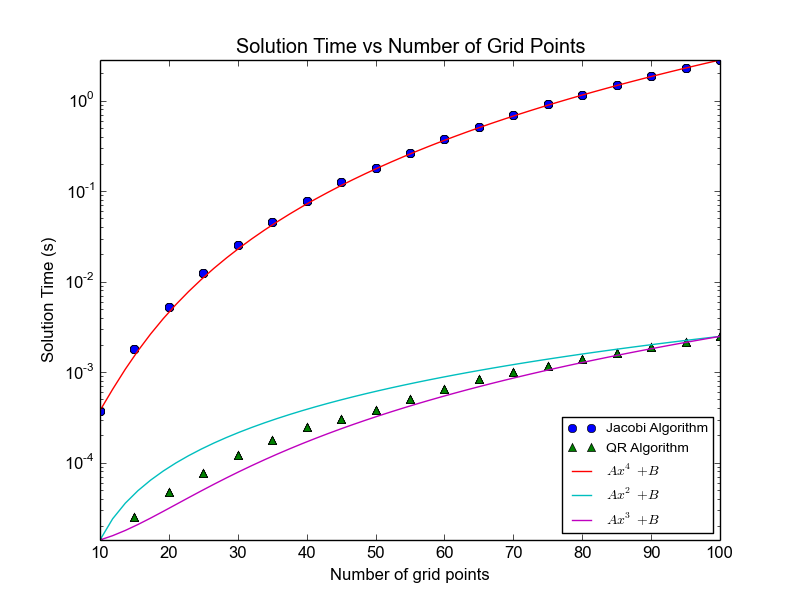
\includegraphics[width=0.6\textwidth]{SeHoTimeTest.png}
 \caption{Plot of the time to converge to a solution versus the number of grid points. Used $\rho_{\mathrm{max}} = 4.61$ with the non-interacting harmonic potential.}
 \label{fig:sehotime}
\end{SCfigure}

The quartic increase in computation time for Jacobi's algorithm is expected. Each rotation requires $~n^2$ operations. Additionally, as we can see in figure (\ref{fig:sehoiter}) that the number of rotations increases as the square of the number of grid points. This is because the number of matrix elements that need to be ``rotated away'' also increases as the square of the number of grid points. Using these facts, we get a computation time that increases like $(n^2)^2 = n^4$.

\begin{SCfigure}
\centering
 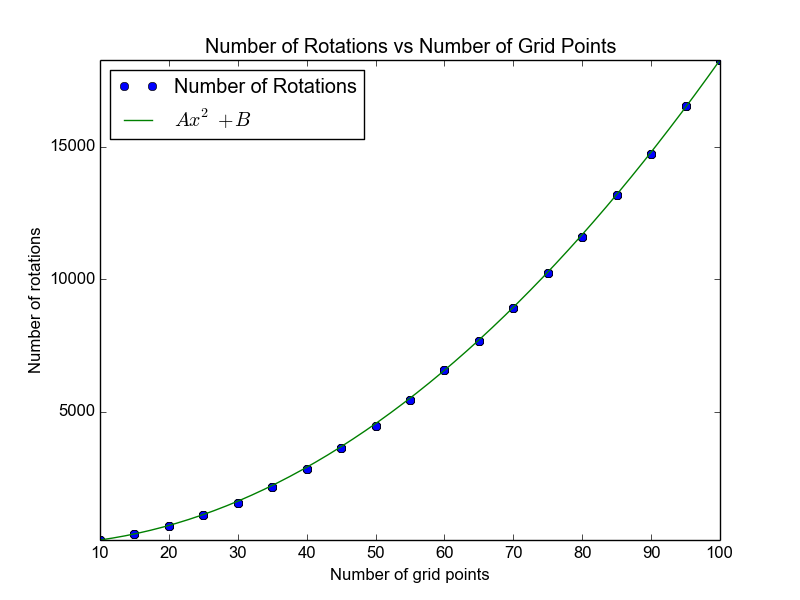
\includegraphics[width=0.6\textwidth]{SeHoIterTest.png}
 \caption{Plot of the number of rotations required for all non-diagonal elements to be zero versus the number of grid points used. Used $\rho_{\mathrm{max}} = 4.61$ with the non-interacting harmonic potential.}
 \label{fig:sehoiter}
\end{SCfigure}

To help evaluate the accuracy of the Jacobi eigenvalue algorithm, a $\chi^2$ test was used
\begin{equation}
 \chi^2 = \sum_{\mathrm{Eigenvalues}}\left(\frac{E_{\mathrm{ana}} - E_{\mathrm{calc}}}{\sigma}\right)^2
\end{equation}
where $E_{\mathrm{ana}}$ and $E_{\mathrm{calc}}$ are the analytical and calculated eigenvalues respectively, and $\sigma$ is the maximum error allowed for an accuracy of 4 significant digits. If most of the eigenvalues in the $\chi^2$ function are accurate to ~4 significant digits, then the $\chi^2$ function should give a result on the order of the number of eigenvalues used in its sum. It was found that such an accuracy is achieved when the number of grid points is about 250. Increasing the number of grid points only increases the resolution of the wave function, so it is expected to see a monotonic decrease in $\chi^2$ with this increase. This is can be seen in figure (\ref{fig:sehontest}). 

\begin{SCfigure}
\centering
 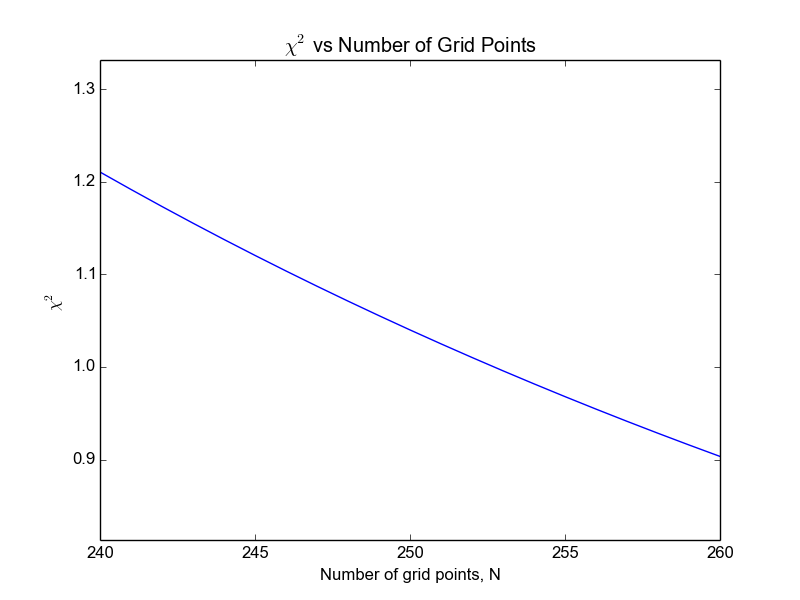
\includegraphics[width=0.6\textwidth]{SeHoNtest.png}
 \caption{Plot of the $\chi^2$ function vs the number of grid points in the region where eigenvalues reach an accuracy of 4 significant digits. Used $\rho_{\mathrm{max}} = 4.61$ with the non-interacting harmonic potential.}
 \label{fig:sehontest}
\end{SCfigure}

It is interesting to note that the accuracy of the calculation for a given number of grid points has a heavy dependence on the maximum range $\rho_{\mathrm{max}}$. If $\rho_{\mathrm{max}}$ is too small, then it is too close to the length scale of the problem and is not a good approximation for infinity. If $\rho_{\mathrm{max}}$ is too large, then all of the interesting features of the wave function are restricted to the beginning of the range of $\rho$, which reduces the number of grid points that contribute to the lower energy eigenfunctions. This dependence can be seen in figure (\ref{fig:sehortest}).

\begin{SCfigure}
\centering
 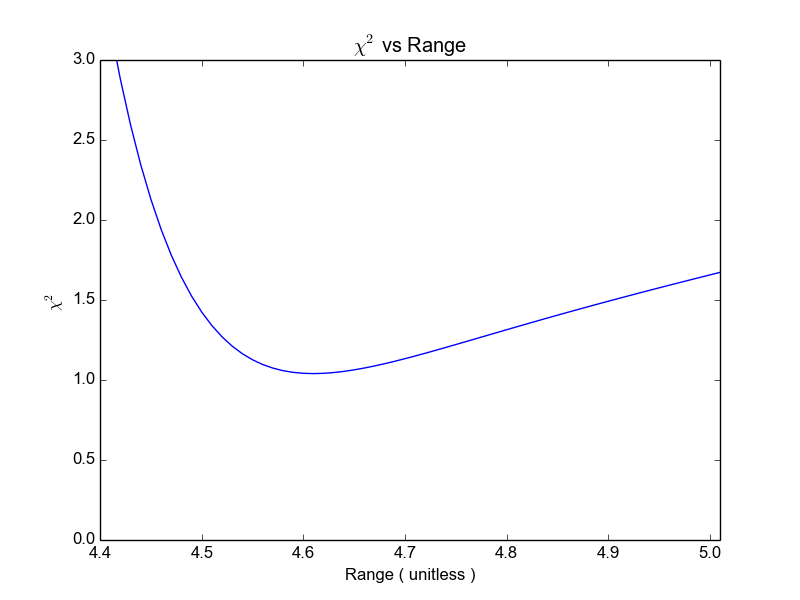
\includegraphics[width=0.6\textwidth]{SeHoRtest.png}
 \caption{Plot of the $\chi^2$ function vs $\rho_{\mathrm{max}}$ in the region where eigenvalues reach an accuracy of 4 significant digits. Used $N = 250$.}
 \label{fig:sehortest}
\end{SCfigure}

It was found that the optimum value for the maximum range with $N = 250$ is $\rho_{\mathrm{max}} = 4.61$. Using these values, the lowest three energy levels for the single electron harmonic oscillator were able to be calculated to 4 significant digits. Their values can be found in table (\ref{tbl:dehoeval}) under the non-interacting case with the $\omega_r$ value of 1, where the expected results are $\lambda = 3,7,11$.

\begin{table}[h]
 \centering
\begin{center}
\begin{tabular}{|c|c|c|c|}\hline
$\mathbf{\omega_r}$ & \textbf{E1} & \textbf{E2} & \textbf{E3}\\\hline
\multicolumn{4}{|c|}{\textbf{Non Interacting}} \\\hline
0.01 & 0.523415 & 1.92596 & 4.249 \\\hline
0.5 & 2.12132 & 4.95436 & 7.87206 \\\hline
1 & 2.99989 & 6.99953 & 11.0016 \\\hline
5 & 6.70768 & 15.6498 & 24.5903 \\\hline
\multicolumn{4}{|c|}{\textbf{Interacting}} \\\hline
0.01 & 0.598781 & 0.968214 & 1.34651 \\\hline
0.5 & 3.00078 & 5.70915 & 8.46232 \\\hline
1 & 4.05769 & 7.90882 & 11.8171 \\\hline
5 & 8.32214 & 17.0252 & 25.8243 \\\hline
\end{tabular}
\end{center}
\caption{Table of the first three energy levels of the (non)interacting double electron harmonic oscillator.\label{tbl:dehoeval}}
\end{table}

The eigenvalue solutions for the interacting case ( equation (\ref{eq:deho}) ) have also been included in table (\ref{tbl:dehoeval}). Exact solutions in this case can be found for some select values of $\omega_r$ in reference \cite{Taut:1993}. The results in table (\ref{tbl:dehoeval}) at least appear to be of the same order of magnitude as these exact solutions. Note that in the non-interacting case, $N=250$ grid points were used with a $\rho_{\mathrm{max}} = 4.61$. These values were only optimal for $\omega_r = 1$, but they were unchanged for the different values of $omega_r$ to see how the wave function is affected for non-optimal values. For the interacting case, $N=250$ grid points were still used, but the range was changed to $\rho_{\mathrm{max}} = 20, 8, 6, 4.61$ for $\omega_r = 0.01,0.5, 1,5$ respectively. These values are not necessarily optimal ( an optimization routine is beyond the scope of this project ), but by looking at the interacting case's wave function plots, we can see they are close to optimal.

To allow for easier comparison, the wave function plots for the interacting and non-interacting cases can be found in appendix (\ref{app:wf}). The wave functions in both cases act as expected, with $n-1$ nodes for the $n^{th}$ energy level. We can see that the optimized case in figure (\ref{fig:se1}) that the interesting features of the wave functions take up the entire range of the plot and smoothly go to zero at $\rho_{\mathrm{max}}$. This can be compared to the non-optimized cases. In figure (\ref{fig:se001}) that for $\omega_r = 0.01$, the longer wavelength wave functions are abruptly cut off at $\rho_{\mathrm{max}}$ without smoothly going to zero ( i.e. $\psi'(\rho_{\mathrm{max}} \neq 0$ ). Conversely, for the short wavelength $\omega_r = 5.0$ in figure (\ref{fig:se001}), we can see that the wave functions all have a magnitude of about zero at $\rho = 3.5$. Hence, the grid points between $\rho = 3.5$ and $\rho_{\mathrm{max}} = 4.61$ are essentially wasted for these lower energy levels. This reduces the number of effective grid points used in calculating the eigensystem, which ultimately causes the accuracy of the energy level calculations to suffer.

Comparing the interacting and non-interacting cases, it was expected that the repulsion between the electrons would cause an upward shift in the energy levels of the system. Looking at table (\ref{tbl:dehoeval}), this is exactly what is seen in most cases. The $\omega_r = 0.01$ case is the exception but, as discussed above, the accuracy in this case is hindered by $\rho_{\mathrm{max}}$ being too small. Little difference is seen in comparing the wave functions of the two cases, but since the energy shift is relatively small -- on the same order as the energy levels themselves -- this is not unexpected. There is a phase difference in the ground state of the interacting case in figures (\ref{fig:de001}) and (\ref{fig:de1}), but since the probability distribution is given as the square of the magnitude of the wave function, this will have no effect on further calculations.

\section{Conclusion}\label{sec:conclusion}
We have shown that Jacobi's eigenvalue algorithm can be used with the discretized Schr\"odinger equation to calculate the solutions to the non-interacting and interacting double electron harmonic oscillator problems to an accuracy that is dependent on the number of grid points used. For a given number of grid points, the accuracy of the calculation has a heavy dependence on the maximum range $\rho_{\mathrm{max}}$. If $\rho_{\mathrm{max}}$ is too small, then interesting features of the wave functions get cut off and are not included in the eigenvalue calculation. If $\rho_{\mathrm{max}}$ is too large, then the wave functions go to zero too soon so the number of effective grid points is reduced. If the actual energy levels are known analytically or experimentally, this could be remedied by using optimization software that minimizes the $\chi^2$ function with respect to $\rho_{\mathrm{max}}$ for a given number of grid points. If the actual energy levels are unknown, we could instead look at the wave functions for a given number of grid points and set $\rho_{\mathrm{max}}$ to the minimum value of $\rho$ where they smoothly go to zero. 

Additionally, in comparing Jacobi's algorithm with the QR algorithm used by GSL it was found that the calculational results were identical, but Jacobi's algorithm had a much longer computation time. Its computation time increased quartically as a function of the number of grid points. GSL's QR algorithm was shown to be much faster, with computation time increasing quadratically or cubically with the number of grid points. As a result, it is not recommended to use Jacobi's eigenvalue algorithm in time intensive calculations.

\appendix
\addtocontents{toc}{\protect\contentsline{chapter}{Appendix:}{}}
\chapter{Wave Function Plots}\label{app:wf}
\begin{SCfigure}
\centering
 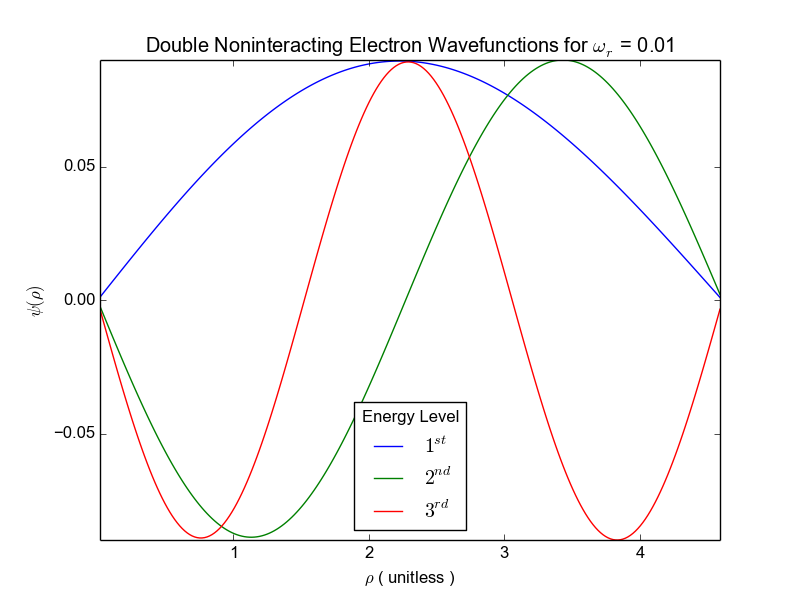
\includegraphics[width=0.6\textwidth]{SeHoWfWr001.png}
 \caption{Plot of the first three non-interacting double electron harmonic oscillator wave functions. $N = 250$, $\rho_{\mathrm{max}} = 4.61$, $\omega_r = 0.01$.}
 \label{fig:se001}
\end{SCfigure}

\begin{SCfigure}
\centering
 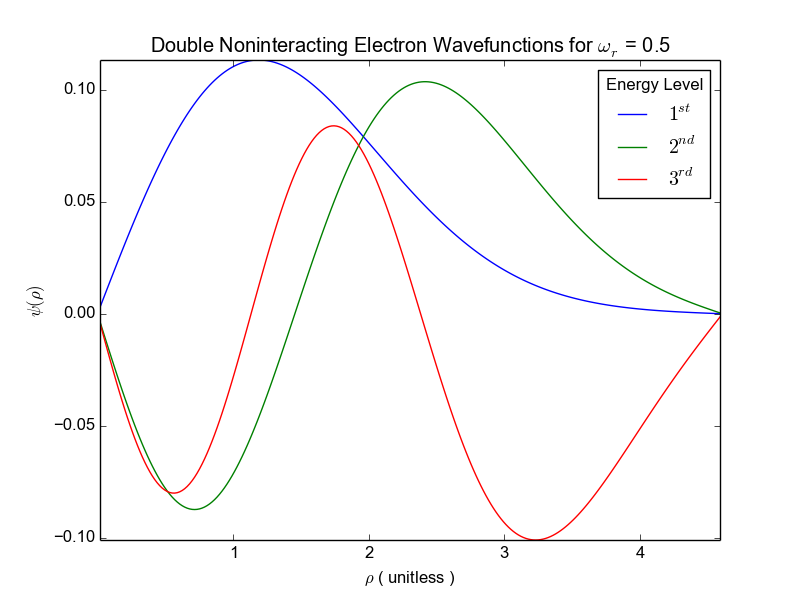
\includegraphics[width=0.6\textwidth]{SeHoWfWr05.png}
 \caption{Plot of the first three non-interacting double electron harmonic oscillator wave functions. $N = 250$, $\rho_{\mathrm{max}} = 4.61$, $\omega_r = 0.5$.}
 \label{fig:se05}
\end{SCfigure}

\begin{SCfigure}
\centering
 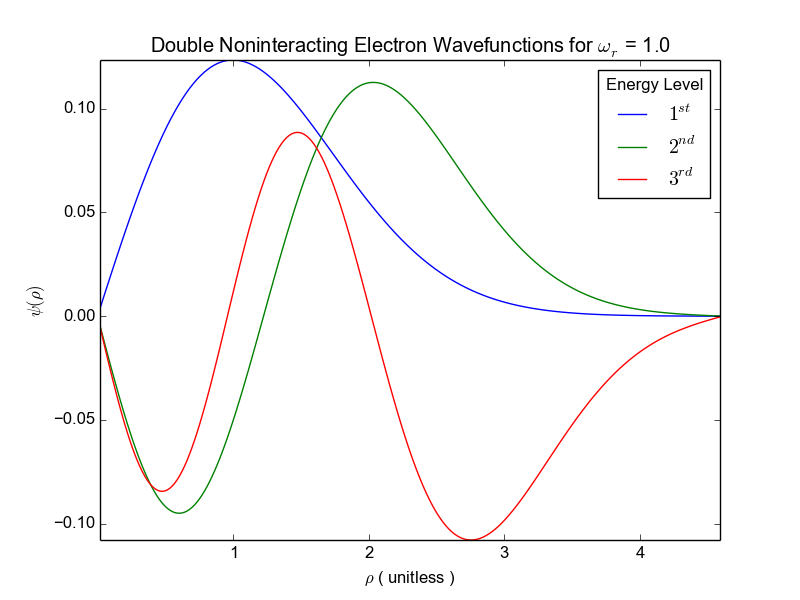
\includegraphics[width=0.6\textwidth]{SeHoWfWr1.png}
 \caption{Plot of the first three non-interacting double electron harmonic oscillator wave functions. $N = 250$, $\rho_{\mathrm{max}} = 4.61$, $\omega_r = 1.0$.}
 \label{fig:se1}
\end{SCfigure}

\begin{SCfigure}
\centering
 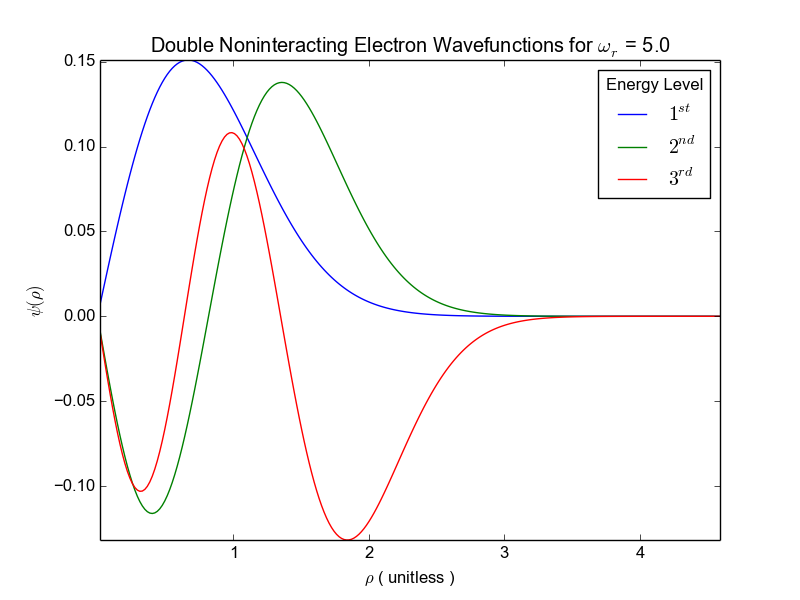
\includegraphics[width=0.6\textwidth]{SeHoWfWr5.png}
 \caption{Plot of the first three non-interacting double electron harmonic oscillator wave functions. $N = 250$, $\rho_{\mathrm{max}} = 4.61$, $\omega_r = 5.0$.}
 \label{fig:se5}
\end{SCfigure}

\begin{SCfigure}
\centering
 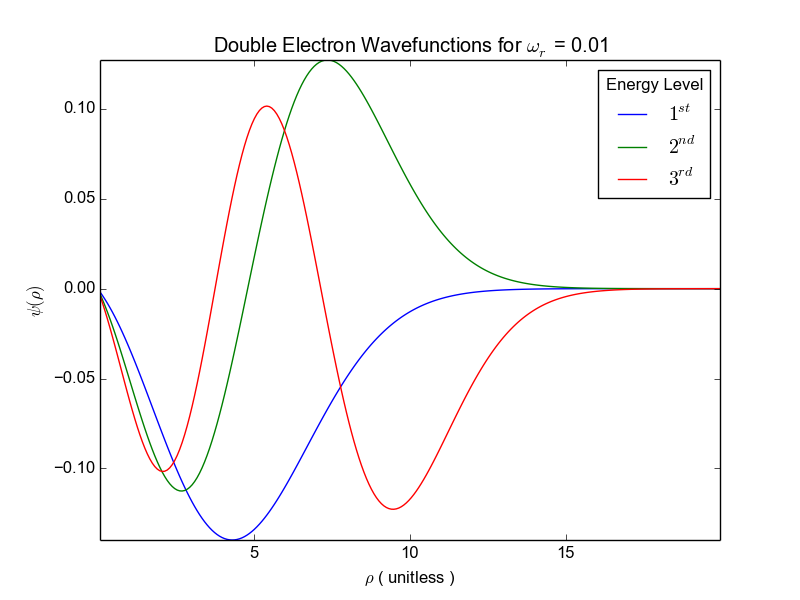
\includegraphics[width=0.6\textwidth]{DeHoWfWr001.png}
 \caption{Plot of the first three interacting double electron harmonic oscillator wave functions. $N = 250$, $\rho_{\mathrm{max}} = 20.0$, $\omega_r = 0.01$.}
 \label{fig:de001}
\end{SCfigure}

\begin{SCfigure}
\centering
 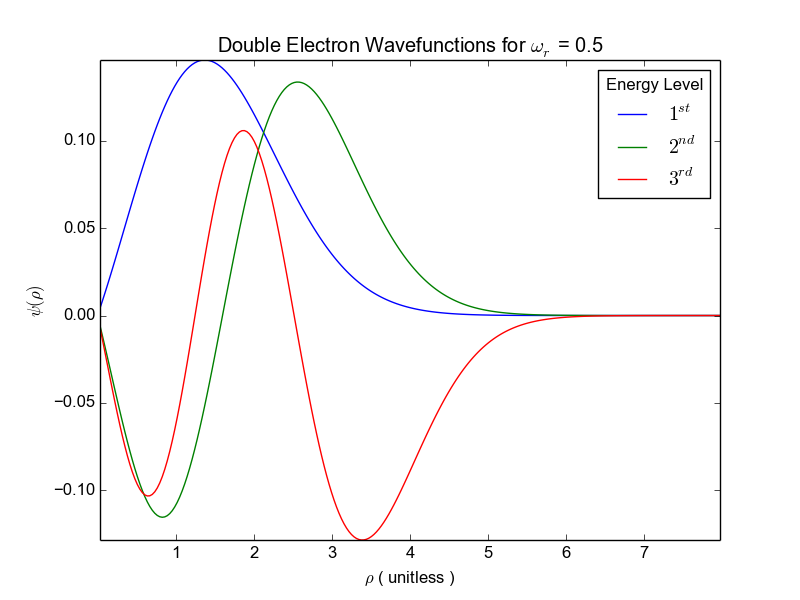
\includegraphics[width=0.6\textwidth]{DeHoWfWr05.png}
 \caption{Plot of the first three interacting double electron harmonic oscillator wave functions. $N = 250$, $\rho_{\mathrm{max}} = 8.0$, $\omega_r = 0.5$.}
 \label{fig:de05}
\end{SCfigure}

\begin{SCfigure}
\centering
 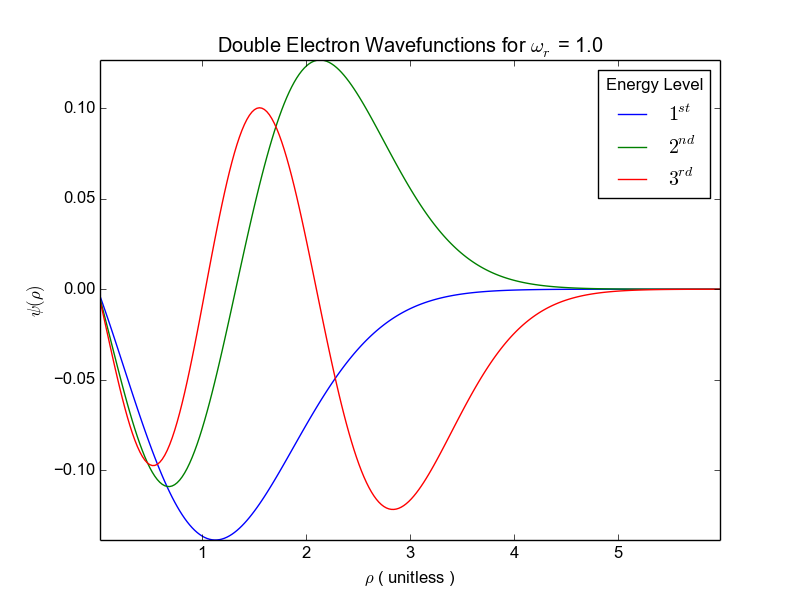
\includegraphics[width=0.6\textwidth]{DeHoWfWr1.png}
 \caption{Plot of the first three interacting double electron harmonic oscillator wave functions. $N = 250$, $\rho_{\mathrm{max}} = 6.0$, $\omega_r = 1.0$.}
 \label{fig:de1}
\end{SCfigure}

\begin{SCfigure}
\centering
 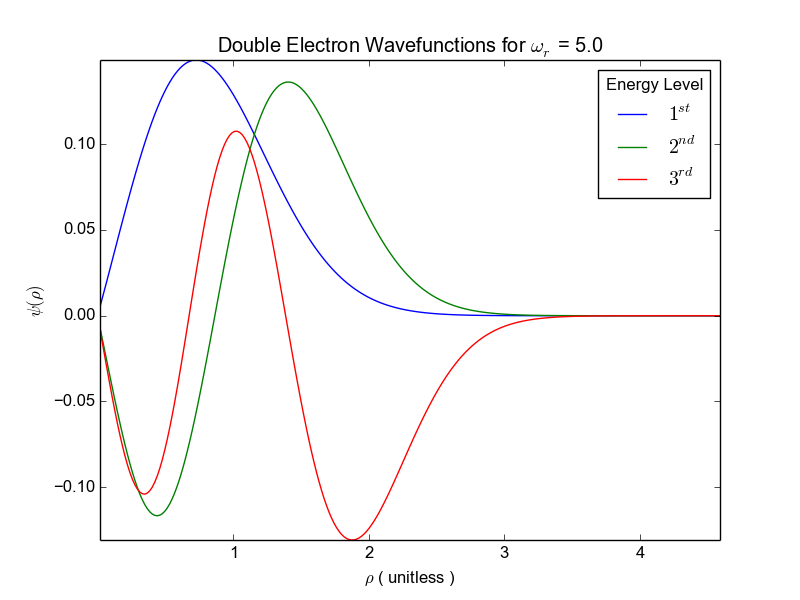
\includegraphics[width=0.6\textwidth]{DeHoWfWr5.png}
 \caption{Plot of the first three interacting double electron harmonic oscillator wave functions. $N = 250$, $\rho_{\mathrm{max}} = 4.61$, $\omega_r = 5.0$.}
 \label{fig:de5}
\end{SCfigure}

\nocite{*}
\bibliographystyle{plain}
\bibliography{ReportProject2.bib}
\end{document}          
